\documentclass[convert={density=300,size=1080x800,outext=.png}]{standalone}

\usepackage{tikz}

\usetikzlibrary{shapes,arrows,positioning,backgrounds,shadows}
% \tikzexternalize
\usetikzlibrary{arrows.meta}

\tikzstyle{decision} = [diamond, draw, fill=white!20, 
    text width=4.5em, text badly centered, node distance=3cm, inner sep=0pt]
\tikzstyle{block} = [rectangle, draw, fill=white!20, 
    text width=8em, text centered, rounded corners, minimum height=2em,node distance=4em]
\tikzstyle{block2} = [rectangle, draw, fill=white!20, 
    text width=8em, text centered, rounded corners, minimum height=2em,node distance=4em,fill=red!20]
\tikzstyle{output} = [rectangle, draw, fill=white!20, 
    text width=8em, text centered, rounded corners, minimum height=2em,node distance=4em,fill=green!20]
% \tikzstyle{easy} = [rectangle, draw, fill=green!40, 
%     text width=5em, text centered, rounded corners, minimum height=4em]
% \tikzstyle{medium} = [rectangle, draw, fill=orange!40, 
%     text width=5em, text centered, rounded corners, minimum height=4em]
% \tikzstyle{hard} = [rectangle, draw, fill=red!40, 
%     text width=5em, text centered, rounded corners, minimum height=4em]
\tikzstyle{line} = [draw, -latex']
\tikzstyle{cloud} = [draw, ellipse,fill=red!20, node distance=3cm,
    minimum height=2em]

\begin{document}
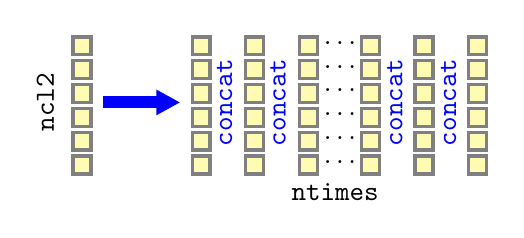
\begin{tikzpicture}
    \node[rotate=90] (ncl2) at (-1em,-4ex) {\texttt{ncl2}};
    \node (ncl2) at (22ex,-11.5ex) {\texttt{ntimes}};

    \foreach \y in {0,1,2,3,4,5}
    {  
        \path (0,\y*-2ex) node (bot_left) {};
        \path (bot_left)+(1.5ex,1.5ex) node (top_right) {};
        \path[draw=black!50,very thick,fill=yellow!30] (bot_left) rectangle (top_right);
    };

    \draw[blue, fill=green, -{Triangle[width = 2ex, length = 2ex]}, line width = 1ex] (2.5ex, -4ex) -- (9ex, -4ex);

    \foreach \y in {0,1,2,3,4,5}
    {  
            \foreach \x in {0,1,2}
            {
                \path (\x*4.5ex+10ex,\y*-2ex) node (bot_left) {};
                \path (bot_left)+(1.5ex,1.5ex) node (top_right) {};
                \path[draw=black!50,very thick,fill=yellow!30] (bot_left) rectangle (top_right);
            };
            \node (dot) at (22.4ex,\y*-2ex+1ex) {$\ldots$};
            \foreach \x in {0,1,2}
            {

                \path (24.2ex+\x*4.5ex,\y*-2ex) node (bot_left) {};
                \path (bot_left)+(1.5ex,1.5ex) node (top_right) {};
                \path[draw=black!50,very thick,fill=yellow!30] (bot_left) rectangle (top_right);
            };
    };
    \node[rotate=90] at (12.7ex,-4ex) {\color{blue}\texttt{concat}};
    \node[rotate=90] at (17.2ex,-4ex) {\color{blue}\texttt{concat}};
    \node[rotate=90] at (27ex,-4ex) {\color{blue}\texttt{concat}};
    \node[rotate=90] at (31.5ex,-4ex) {\color{blue}\texttt{concat}};
\end{tikzpicture}
\end{document}